\documentclass[letterpaper]{article}

\usepackage{multicol}
\usepackage{geometry}
\usepackage{hyperref}
\usepackage{graphicx}
\usepackage{booktabs}
\usepackage{caption}

\graphicspath{ {assets/} }

\geometry{margin=1in}

% Title
\title{Heuristic Analysis}
\author{Kyung Mo Kweon}
\date{\today}

% Document
\begin{document}
% Title
\maketitle

% Abstract
\begin{abstract}
This is a summary writeup for \href{https://github.com/kkweon/AIND-Planning}{AIND Project 3 Planning}. This summary consists of three portions. The first portion of this summary is to compare uninformed search algorithms for air cargo problems. The second portion is to compare heuristics search algorithms such as the A* algorithm. The last part is to summarize all and compare heuristics and non-heuristics searches.
\end{abstract}

\section{Uninformed Planning Search}
I ran the following uninformed planning search algorithms to solve air cargo problems.
\begin{itemize}
\item Bredth First Ssearch (BFS)
\item Breadth First Tree Search (BF-Tree-S)
\item Depth First Graph Search (DF-Graph-S)
\item Depth Limited Search (D-Limited-S) 
\end{itemize}
BF-Tree-Search failed to find a solution for air cargo prolbem 2 and 3 within 10 minutes, which results in NaN. Depth-Limited-Search also failed to find a solution for the problem 3.
\autoref{table:usa} and \autoref{fig:usa} shows the detailed information such as number of node expnaded, running time, etc.

\subsection*{Solution Path}
BFS was able to find the optimal solution for each problem. This is a solution found by BFS. 
\begin{multicols}{3}

\begin{verbatim}
For air cargo problem 1,

Load(C2, P2, JFK) 
Load(C1, P1, SFO) 
Fly(P2, JFK, SFO)  
Unload(C2, P2, SFO) 
Fly(P1, SFO, JFK) 
Unload(C1, P1, JFK) 
\end{verbatim}
\columnbreak

\begin{verbatim}
For air cargo problem 2, 

Load(C1, P1, SFO) 
Load(C2, P2, JFK)  
Load(C3, P3, ATL) 
Fly(P1, SFO, JFK) 
Unload(C1, P1, JFK) 
Fly(P2, JFK, SFO) 
Unload(C2, P2, SFO) 
Fly(P3, ATL, SFO)  
Unload(C3, P3, SFO) 
\end{verbatim}
\columnbreak

\begin{verbatim}
For air cargo problem 3, 

Load(C1, P1, SFO)
Load(C2, P2, JFK)
Fly(P1, SFO, ATL)
Load(C3, P1, ATL)
Fly(P2, JFK, ORD)
Load(C4, P2, ORD)
Fly(P1, ATL, JFK)
Unload(C1, P1, JFK)
Unload(C3, P1, JFK)
Fly(P2, ORD, SFO)
Unload(C2, P2, SFO)
Unload(C4, P2, SFO)
\end{verbatim} 
\end{multicols}

\subsection*{Summary}
In summary, BFS is the best bet to use although DF-Graph-Search tends to expand less number of nodes which result in a quicker run because Depth first approach only looks at the current node and if it's the goal node, it will stop right there.

\begin{table}
\begin{tabular}{rlrrrrr}
\toprule
 problem &  search\_type &  expansions &  goal\_tests &  new\_nodes &  plan\_length &     seconds \\
\midrule
       1 &          BFS &          43 &          56 &        180 &            \textbf{6} &    0.020423 \\
       1 &    BF-Tree-S &        1,458 &        1,459 &       5,960 &            6 &    0.639505 \\
       1 &   DF-Graph-S &          \textbf{12} &          \textbf{13} &         \textbf{48} &           12 &    \textbf{0.005444} \\
       1 &  D-limited-S &         101 &         271 &        414 &           50 &    0.059900 \\
\midrule
       2 &          BFS &        3,346 &        4,612 &      30,534 &            \textbf{9} &    9.245823 \\
       2 &    BF-Tree-S &         - &         - &        - &          - &         - \\
       2 &   DF-Graph-S &        \textbf{1,124} &        \textbf{1,125} &      \textbf{10,017} &         1,085 &    \textbf{5.271785} \\
       2 &  D-limited-S &       13,491 &     1,967,093 &    1,967,471 &           50 &  586.502468 \\
\midrule
       3 &          BFS &       14,120 &       17,673 &     124,926 &           \textbf{12} &   66.104630 \\
       3 &    BF-Tree-S &         - &         - &        - &          - &         - \\
       3 &   DF-Graph-S &         \textbf{677} &         \textbf{678} &       \textbf{5608} &          660 &    \textbf{2.407824} \\
       3 &  D-limited-S &         - &         - &        - &          - &         - \\
\bottomrule
\end{tabular}
\caption{Comparison of uninformed search algorithms. Each columns means number of nodes, `-' implies it was unable to find a solution in 10 minutes. Only BFS was able to find optimal solutions.}
\label{table:usa}
\end{table}

\begin{figure}
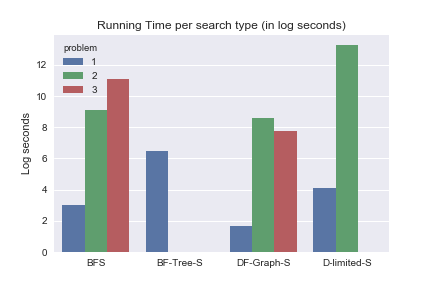
\includegraphics[scale=1]{assets/uninformed_search.png}
\caption{Running time of uninformed search algorithms in log seconds. BFS seems to work the best for all 3 cargo problems. DF-graph-search ran the quickest although it did not return the optimal solution.}
\label{fig:usa}
\end{figure}

\newpage
\section{Informed Planning Search: Domain Independent Heuristics}
I have tested following 3 different A* searches:
\begin{itemize}
\item Recursive Best First Search with h1 (Recursive h1)
\item Greedy Best First Graph Search with h1 (Greedy h1)
\item A* with h1 (A* h1)
\item A* with h\_ignore\_preconditions (A* h\_ignore)
\item A* with h\_pg\_levelsum (A* h\_levelsum)
\end{itemize}

and each heuristics $h$ means the following:
\begin{itemize}
       \item h1: it always returns 1
       \item h\_ignore\_precondtions: it ignores preconditions of actions and counts the number of actions to take to reach a goal state 
       \item h\_pg\_levelsum: it uses the state spaces and sums up the number of actions in a state level
\end{itemize}

Every A* algorithms is able to find an optimal policy because the heuristics functions used here are admissible, which means heuristics functions return less cost than its actual cost while others do not necessarily return optimal solutions.
\autoref{table:informed} and \autoref{fig:informed} shows the detailed information.

\subsection*{Solution Path}
This is a solution found by A* with ignore precondition heuristics. 
\begin{multicols}{3}

\begin{verbatim}
For air cargo problem 1,

Load(C1, P1, SFO)
Fly(P1, SFO, JFK)
Unload(C1, P1, JFK)
Load(C2, P2, JFK)
Fly(P2, JFK, SFO)
Unload(C2, P2, SFO)
\end{verbatim}
\columnbreak

\begin{verbatim}
For air cargo problem 2, 

Load(C3, P3, ATL)
Fly(P3, ATL, SFO)
Unload(C3, P3, SFO)
Load(C2, P2, JFK)
Fly(P2, JFK, SFO)
Unload(C2, P2, SFO)
Load(C1, P1, SFO)
Fly(P1, SFO, JFK)
Unload(C1, P1, JFK)
\end{verbatim}
\columnbreak

\begin{verbatim}
For air cargo problem 3, 

Load(C2, P2, JFK)
Fly(P2, JFK, ORD)
Load(C4, P2, ORD)
Fly(P2, ORD, SFO)
Unload(C4, P2, SFO)
Load(C1, P1, SFO)
Fly(P1, SFO, ATL)
Load(C3, P1, ATL)
Fly(P1, ATL, JFK)
Unload(C3, P1, JFK)
Unload(C2, P2, SFO)
Unload(C1, P1, JFK)
\end{verbatim} 

\end{multicols}
\subsection*{Summary}
In summary, the best informed search algorithm is to use A* with ignore precondition heuristics because it was able to find all solutions and return the optimal solution.
Interestingly, greedy search was the fastest except for problem 3 because like DFS case, it does not search for an optimal solution and thus runs quicker.


\begin{table}[!ht]
\begin{tabular}{rlrrrrr}
\toprule
 problem &    search\_type & expansions & goal\_tests & new\_nodes & plan\_length &     seconds \\
\midrule
       1 &   Recursive h1 &      4,229 &      4,230 &    17,029 &           6 &    2.192055 \\
       1 &      Greedy h1 &          \textbf{7} &          \textbf{9} &        \textbf{28} &           \textbf{6} &    \textbf{0.003459} \\
       1 &          A* h1 &         55 &         57 &       224 &           6 &    0.026202 \\
       1 &    A* h\_ignore &         41 &         43 &       170 &           6 &    0.021445 \\
       1 &  A* h\_levelsum &         11 &         13 &        50 &           6 &    0.977602 \\
\midrule
       2 &   Recursive h1 &        - &        - &       - &         - &         - \\
       2 &      Greedy h1 &        998 &      1,000 &     8,982 &          21 &    \textbf{4.889845} \\
       2 &          A* h1 &      4,853 &      4,855 &    44,041 &           9 &   30.183343 \\
       2 &    A* h\_ignore &      1,506 &      1,508 &    13,820 &           9 &    8.495319 \\
       2 &  A* h\_levelsum &         \textbf{86} &         \textbf{88} &       \textbf{841} &           \textbf{9} &  100.212704 \\
\midrule
       3 &   Recursive h1 &        - &        - &       - &         - &         - \\
       3 &      Greedy h1 &      5,578 &      5,580 &    49,150 &          22 &   64.216118 \\
       3 &          A* h1 &     18,223 &     18,225 &   159,618 &          12 &  249.243397 \\
       3 &    A* h\_ignore &      \textbf{5,118} &      \textbf{5,120} &    \textbf{45,650} &          \textbf{12} &   \textbf{54.246282} \\
       3 &  A* h\_levelsum &        - &        - &       - &         - &         - \\
\bottomrule
\end{tabular}
\caption{Informed Search Result: `-' indicates the search did not return a solution within 10 minutes. A* with ignore precondtions seems to work the best because levelsum heuristics failed to find a solution within the time limit.}
\label{table:informed}
\end{table}

\begin{figure}[!ht]
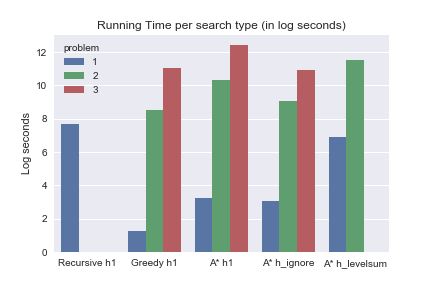
\includegraphics[scale=1]{assets/informed_search.png}
\caption{Running time of informed search algorithms in log seconds. Among A* searches, the ignore precondition heuristics is likely the best choice. Running time wise, greedy h1 seems the quickest except for problem 3 although it did not return the optimal solution.}
\label{fig:informed}
\end{figure}

\newpage\phantom{ss}
\section{Conclusion}
In this section, I will try to answer questions on \href{https://github.com/udacity/AIND-Planning}{\texttt{README.md}}

\subsection*{Provide optimal plans for P1, P2, P3}
It was mentioned already above in Solution Path.

\subsection*{Compare and contrast non-heuristic search result metrics}
Only BFS was able to find optimal solutions although depth first graph search was able to return a (non-optimal) solution quicker due to the fact that it only looks at the current node and does not look for an optimal path.
BF-Tree-Search and Depth-Limited-Search failed to return solutions for problem 2 and problm 3 within 10 minutes limit.

Please refer to \autoref{table:usa} and \autoref{fig:usa}.

\subsection*{Compare and contrast heuristic search result metrics}
Between ``ignore precondtion'' and ``level sum'' heuristics, it's advised to use ignore precondtions heuristics because the level sum heuristics failed to return a solution for problem 3 within the time limit.
The ignore precondition heuristics returns an optimal solution because the heuristic is admissible.

Please refer to \autoref{table:informed} and \autoref{fig:informed}

\subsection*{Best Heuristics vs Best Non Heuristics}
From previous sections, I concluded BFS works the best for finding an optimal solution and DF-Graph-Search is the quickest for non heuristics search. For heuristic searches, A* with ignore precondtion heuristics was able to find an optimal solution for all 3 problems efficiently.

Below is the comparison between the best non heuristics searches (BFS and DF-Graph-Search) and the best heuristics search (A* search).

\begin{table}[!h]
\begin{tabular}{rlrrrrr}
\toprule
 problem &                     search\_type & expansions & goal\_tests & new\_nodes & plan\_length &    seconds \\
\midrule
       1 &                             BFS &         43 &         56 &       180 &           \textbf{6} &   0.020423 \\
       1 &                      DF-Graph-S &         \textbf{12} &         \textbf{13} &        \textbf{48} &          12 &   \textbf{0.005444} \\
       1 &  A* with h\_ignore\_preconditions &         41 &         43 &       170 &           \textbf{6} &   0.021445 \\
\midrule
       2 &                             BFS &      3,346 &      4,612 &    30,534 &           \textbf{9} &   9.245823 \\
       2 &                      DF-Graph-S &      \textbf{1,124} &      \textbf{1,125} &    \textbf{10,017} &       1,085 &   \textbf{5.271785} \\
       2 &  A* with h\_ignore\_preconditions &      1,506 &      1,508 &    13,820 &           \textbf{9} &   8.495319 \\
\midrule
       3 &                             BFS &     14,120 &     17,673 &   124,926 &          \textbf{12} &  66.104630 \\
       3 &                      DF-Graph-S &        \textbf{677} &        \textbf{678} &     \textbf{5,608} &         660 &   \textbf{2.407824} \\
       3 &  A* with h\_ignore\_preconditions &      5,118 &      5,120 &    45,650 &          \textbf{12} &  54.246282 \\
\bottomrule
\end{tabular}
\end{table}
In conclusion, if I want an optimal solution, I would recommend using the A* with ignore precondition heuristics because its heuristics is admissible and visit less nodes than BFS. However, if I want the quickest search, DF-Graph-Search would be the best to use because it does not care if the solution is optimal.

\end{document}